Es stehen ein RLC-Messgerät, ein Oszilloskop und ein Funktionsgenerator zur Verfügung, sowie einige Koaxialkabel und unbekannte Widerstände in einer Box.
Zunächst werden die \textbf{Messung der Leitungskonstanten $R,L,C$} gemessen. Dafür wird ein Koaxialkabel mit einem Widerstand von \SI{50}{\ohm} an den Funktionsgenerator angeschlossen und mit dem RLC-Messgerät werden die Induktivität, der ohmsche Widerstand und die Kapazität des Kabels bei verschiedenen Frequenzen im Bereich von 0.2-\SI{100}{\kilo\hertz} gemessen. Dieser Schritt wird für ein weiteres Koaxialkabel mit \SI{75}{\ohm} wiederholt. \\
\ \\
Abbildung \ref{fig:Aufbau} zeigt den Aufbau der restlichen Messungen. Ab hier wird nur noch das Kabel mit den \SI{50}{\ohm} verwendet.
\begin{figure}[h]
	\centering
	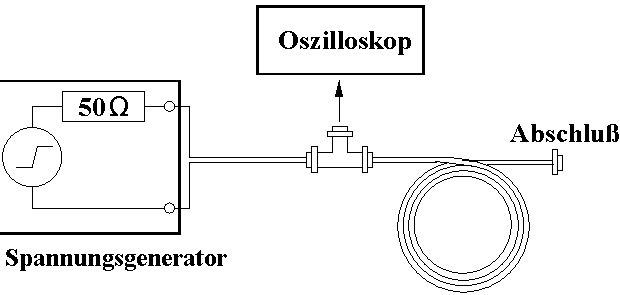
\includegraphics[width=0.4\textwidth]{Aufbau.pdf}
	\caption{Versuchsaufbau \cite{E2}}
	\label{fig:Aufbau}
\end{figure}
\subsubsection*{Messung zur Bestimmung der Dämpfungskonstante}
Um die Dämpfungskonstante bestimmen zu können, wird zuerst ein langes Kabel an den Funktionsgenerator angeschlossen. Am Oszilloskop wird die Fouriertransformierte des Signals angezeigt und ein Bild aufgenommen. Dasselbe wird für ein kurzes Kabel gemacht. Die höheren Moden werden stärker gedämpft als die niedrigen, sodass aus dem Verhältnis der Fourierkoeffizienten der höheren Moden die Dämpfungskonstante bestimmt werden kann.
\subsection*{Messung 3}
Hierzu fehlen die Bilder im Oszilloskop-Ordner.
\subsection*{Abschlusswiderstände}
Der Abschluss des Koaxialkabels wird in drei verschiedene Anschlüsse der Box mit den Widerständen gesteckt und dabei die Signalspannung in Abhängigkeit von der Zeit am Oszilloskop betrachtet. Die aufgenommenen Kurven werden gespeichert. Die Form der Kurven kann dann mit den Kurven in Abbildung \ref{fig:Zeitkonstanten} verglichen werden und so auf den Abschlusswiderstand geschlossen werden.
\subsection*{Mehrfachreflexion}
Durch Reihenschaltung der Kabel mit \SI{50}{\ohm} und \SI{75}{\ohm} kann eine Mehrfachreflexion erzeugt werden. Auch hier fehlt das Bild.